\documentclass[10pt,a4paper]{article}
\usepackage[utf8]{inputenc}
\usepackage{times}
\usepackage{courier}
\usepackage{graphicx}
\usepackage{hyperref}

\title{Implementační dokumentace k \textbf{1}. úloze do IPP 2023/2024}
\author{Jméno a příjmení: \textbf{Jakub Všetečka} \\ Login: \textbf{xvsete00}}
\date{}

\begin{document}

\maketitle

\section{Design Philosophy}
The script is designed with an emphasis on modular architecture and object-oriented principles. The system comprises various classes like XMLGenerator, Argument, Instruction, ArgumentParser, and InstructionParser, each serving a distinct role, thereby promoting code reuse and ease of maintenance. Emphasis is laid on developing a robust solution that adheres to the requirements while maintaining flexibility for future extensions.

\section{Internal Representation}
Each script component is represented as an object. XMLGenerator handles the XML structure, creating a skeleton for the output file. Instructions and their arguments, encapsulated within their respective classes, act as building blocks for the script's functionality. The ArgumentParser and InstructionParser manage input parsing, transforming text into structured data. Enums ensure consistency in defining argument types and instruction formats, aiding in clear, manageable code. These objects are more closely detailed in the class
diagram~\ref{fig:classes}.

\begin{figure}[h]
    \centering
    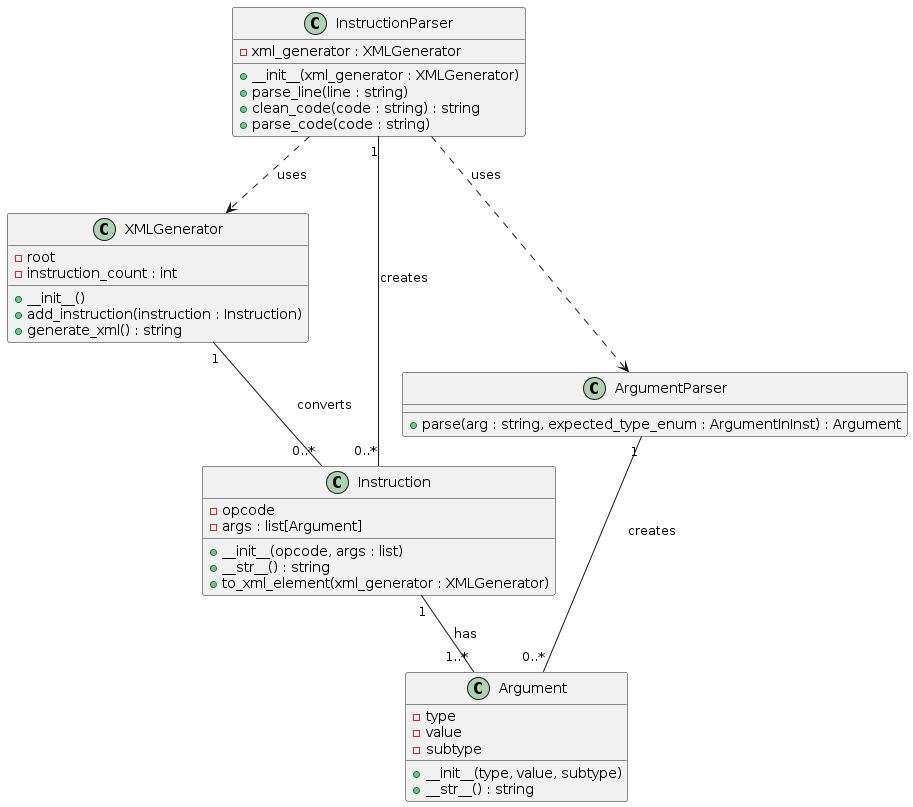
\includegraphics[width=\textwidth]{imgs/classes.png}
    \caption{Class Diagram}
    \label{fig:classes}
    \end{figure}


\section{Solution Procedure}
The approach involves parsing the input, building an internal representation, and outputting an XML document. The script cleans the input to remove extraneous elements like comments, using InstructionParser. It then parses the instructions into objects. XMLGenerator utilizes these objects to construct an XML file. Special attention is given to error handling, particularly for scenarios not explicitly covered in the brief, ensuring the script's reliability. While the implementation doesn't currently employ design patterns, it is structured to allow easy integration in the future.

\end{document}
